\documentclass[a4paper,10pt]{article}
\usepackage[dvips]{color,graphicx}
\usepackage[dvips, bookmarks, colorlinks=false]{hyperref}
\addtolength{\textheight}{8cm}
\addtolength{\textwidth}{3.5cm}
\addtolength{\hoffset}{-2cm}
\addtolength{\voffset}{-3cm}
\setlength{\parskip}{3ex plus 0.5ex minus 0.2ex}


%opening
\title{Math508 Homework 3}
\author{Yu Huang}
\date{2007-02-01}

\begin{document}

\maketitle

\begin{abstract}
Simulation of simple random walk with absorption on Z[0,20].
\end{abstract}

\section{Figures}
\begin{figure}[h]
\includegraphics[width=1\textwidth]{hw3_1_a_N200_X0_5.eps}
\caption{}
\end{figure}
\begin{figure}[p]
\includegraphics[width=1\textwidth]{hw3_1_a_N1000_X0_5.eps}
\caption{}
\end{figure}
\begin{figure}[p]
\includegraphics[width=1\textwidth]{hw3_1_a_N2000_X0_5.eps}
\caption{}
\end{figure}
\begin{figure}
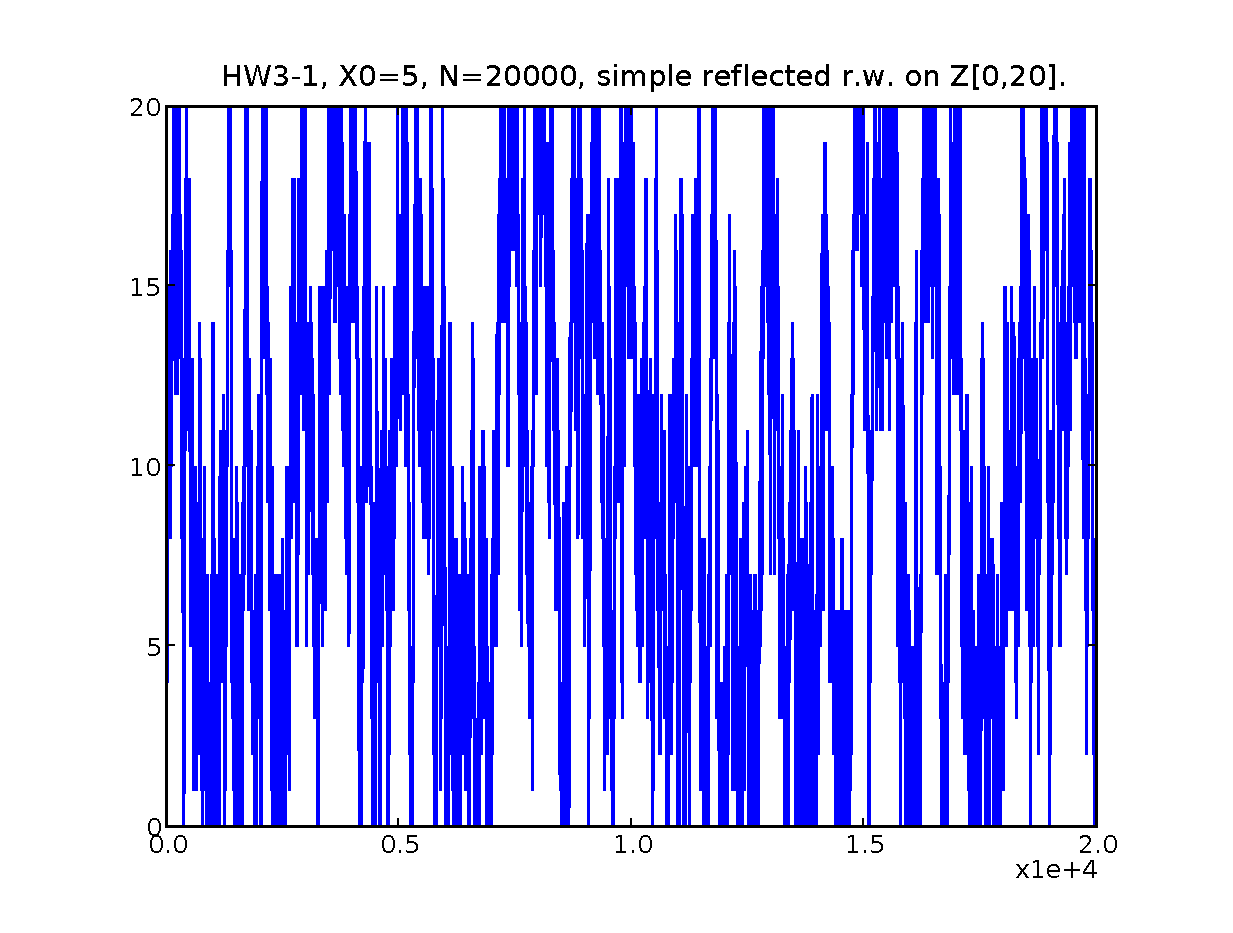
\includegraphics[width=1\textwidth]{hw3_1_a_N20000_X0_5.eps}
\caption{}
\end{figure}
\begin{figure}
\includegraphics[width=1\textwidth]{hw3_1_b_N50_X0_10.eps}
\caption{}
\end{figure}

\begin{figure}
\includegraphics[width=1\textwidth]{hw3_1_b_N100_X0_10.eps}
\caption{}
\end{figure}

\begin{figure}
\includegraphics[width=1\textwidth]{hw3_1_b_N150_X0_10.eps}
\caption{}
\end{figure}

\end{document}
